\itemhead{复习题三 · 第15题（教材p.91）}{XJ-B1-C03-RV-P091-Y1481}
\label{XJ-B1-C03-RV-P091-Y1481}
{\footnotesize 湘教版教材p.91 / PDF第98页 / 复习题三 / 第15题}
\field{原题}{已知某函数在区间 $(-\infty,1]$ 上单调递减，在区间 $[1,+\infty)$ 上单调递增，且 $f(1)=1$。试写出一个这样的函数解析式。}
\field{参考答案}{例如 $f(x)=(x-1)^2+1$，或 $f(x)=|x-1|+1$，均满足；答案不唯一。}
\begin{center}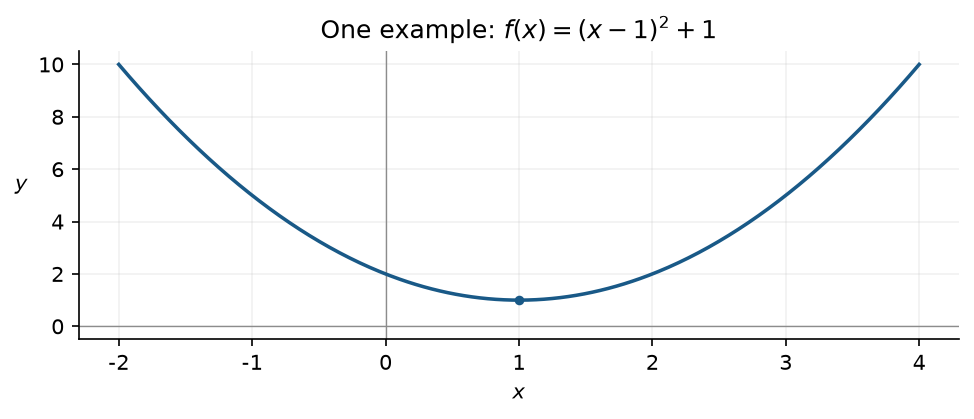
\includegraphics[width=.84\linewidth,height=.38\textheight,keepaspectratio]{figures/C03-RV091-15.png}\end{center}
{\small \field{关联知识}{F05 单调性定义、证明与参数（教材帮p.97、98、100 / PDF106、107、109）；F06 最大值、最小值与值域（教材帮p.99、83、84 / PDF108、92、93）}
\field{方法与易错点}{用定义比较任意两值，或依据已知图象性质；含参时使指定区间被相应单调区间覆盖。 易错：用有限采样代替证明；把分离半轴合并；漏跨零点情形。}
\field{答案依据}{答案册相关题组：PDF第24、25、26、27页（册内页23、24、25、26）；按当前题库原题逐项重算，不按旧版题号机械对套。}}
